\chapter{Application-Aware Techniques to Reduce Offered Load}
\label{chapter: load}

{\em Elasticity} is a key attribute of cloud computing.  When load
rises, new servers can be rapidly spun up.  When load subsides, idle
servers can be quiesced to save energy.  Elasticity is vital to
scalability, because it ensures acceptable response times under a wide
range of operating conditions.  To benefit, cloud services need to be
architected to easily scale out to more servers.  Such a design is
said to be ``cloud-native.''

In contrast, edge computing has limited elasticity.  As its name implies, a
cloudlet is designed for much smaller physical space and electrical power than a
cloud data center.  Hence, the sudden arrival of an unexpected flash crowd can
overwhelm a cloudlet.  Since low end-to-end latency is a prime reason for edge
computing, shifting load elsewhere (e.g., the cloud) is not an attractive
solution.  {\em How do we build multi-user edge computing systems that preserve
low latency even as load increases?}  That is the focus of the next two chapters.

Our approach to scalability is driven by the following observation. Since
compute resources at the edge cannot be increased on demand, the only paths to
scalability are (a) to reduce offered load, as discussed in this chapter,
or (b) to reduce queueing delays through improved end-to-end scheduling,
as discussed in Chapter~\ref{chapter: cloudlet}.  Otherwise, the mismatch between
resource availability and offered load will lead to increased queueing delays
and hence increased end-to-end latency.  Both paths require the average burden
placed by each user on the cloudlet to fall as the number of users increases.
This, in turn, implies {\em adaptive application behavior} based on guidance
received from the cloudlet or inferred by the user's mobile device.  In the
context of Figure~\ref{fig:3tier}, scalability at the left is achieved very
differently from scalability at the right.  The relationship between Tier-3 and
Tier-2 is {\em non-workload-conserving}, while that between Tier-1 and other
tiers is workload-conserving.

While we demonstrated application-agnostic techniques to reduce network
transmission between Tier-3 and Tier-2 in Chapter~\ref{chapter: bandwidth},
offered load can be further reduced with application assistance. We claim that
scalability at the edge can be better achieved for applications that have been
designed with this goal in mind.  We refer to applications that are specifically
written to leverage edge infrastructure as {\em edge-native applications.} These
applications are deeply dependent on the services that are only available at the
edge (such as low-latency offloading of compute, or real-time access to video
streams from edge-located cameras), and are written to adapt to
scalability-relevant guidance.  For example, an application at Tier-3 may be
written to offload object recognition in a video frame to Tier-2, but it may
also be prepared for the return code to indicate that a less accurate (and hence
less compute-intensive) algorithm than normal was used because Tier-2 is heavily
loaded.  Alternatively, Tier-2 or Tier-3 may determine that the wireless channel
is congested; based on this guidance, Tier-3 may reduce offered load by
preprocessing a video frame and using the result to decide whether it is
worthwhile to offload further processing of that frame to the cloudlet.  Several
earlier work~\cite{Hu2015, christensen2019towards} have shown that even
modest computation, such as color filtering and shallow DNN processing, at Tier-3
can make surprisingly good predictions about whether a specific use of Tier-2 is
likely to be worthwhile.

Edge-native applications may also use {\em cross-layer adaptation
  strategies,} by which knowledge from Tier-3 or Tier-2 is used in the
management of the wireless channel between them.  For example, an
assistive augmented reality (AR) application that verbally guides a
visually-impaired person may be competing for the wireless channel and
cloudlet resources with a group of AR gamers.  In an overload
situation, one may wish to favor the assistive application over the
gamers.  This knowledge can be used by the cloudlet operating system
to preferentially schedule the more important workload.  It can also
be used for prioritizing network traffic by using {\em fine-grain
  network slicing,} as envisioned in 5G~\cite{Contreras2018}.

Wearable cognitive assistance, perceived to be ``killer apps'' for edge
computing, are perfect exemplars of edge-native applications. In the rest of
this chapter, we showcase how we can leverage unique application characteristics
of WCAs to adapt application behavior and reduce offered load. Our work is built
on the Gabriel platform~\cite{ha2014towards,chen2017empirical}, shown in
Figure~\ref{fig:gabriel}. The Gabriel front-end on a wearable device performs
preprocessing of sensor data (e.g., compression and encoding), which it streams
over a wireless network to a cloudlet. We refer to the Gabriel platform with new
mechanisms that handle multitenancy, perform resource allocation, and support
application-aware adaptation as ``Scalable Gabriel'' and the single-user
baseline platform as ``Original Gabriel''.

% The Gabriel back-end on the cloudlet has
% a modular structure. The {\em control module} is the focal point for all
% interactions with the wearable device.  A publish-subscribe (PubSub) mechanism
% decodes and distributes the incoming sensor streams to multiple {\em cognitive
% modules} (e.g., task-specific computer vision algorithms) for concurrent
% processing. Cognitive module outputs are integrated by a task-specific {\em user
% guidance module} that performs higher-level cognitive processing such as
% inferring task state, detecting errors, and generating guidance in one or more
% modalities (e.g., audio, video, text, etc.).

% It did,
% however, have a token-based transmission mechanism.  This limited a client to
% only a small number of outstanding operations, thereby offering a simple form of
% rate adaptation to processing or network bottlenecks.  We have retained this
% token mechanism in our system. In addition, 


% Since the techniques for reducing offered workload are application-specific, we
% focus on a specific class of edge-native applications to validate our ideas.
% Our choice is a class of applications called {\em Wearable Cognitive Assistance}
% (WCA) applications~\cite{ha2014towards}.  They are perceived to be ``killer apps'' for
% edge computing because (a) they transmit large volumes of video data to the
% cloudlet; (b) they have stringent end-to-end latency requirements; and (c) they
% make substantial compute demands of the cloudlet, often requiring high-end GPUs.

% We leverage unique characteristics of WCA applications to reduce
% offered load through graceful degradation and improved resource
% allocation.  Our contributions are as follows:
% \begin{smitemize}
%   \item{An architectural framework for WCA that enables graceful degradation under heavy load.}
%   \item{An adaptation taxonomy of WCA applications, and techniques for workload reduction.}
%   \item{A cloudlet resource allocation scheme based on degradation heuristics and external policies.}
%   \item{A prototype implementation of the above.}
%   \item{Experimental results showing up to 40\% reduction in offered load and graceful degradation in oversubscribed edge systems.}
% \end{smitemize}

\section{Adaptation Architecture and Strategy}

\begin{figure}[h]
\centering
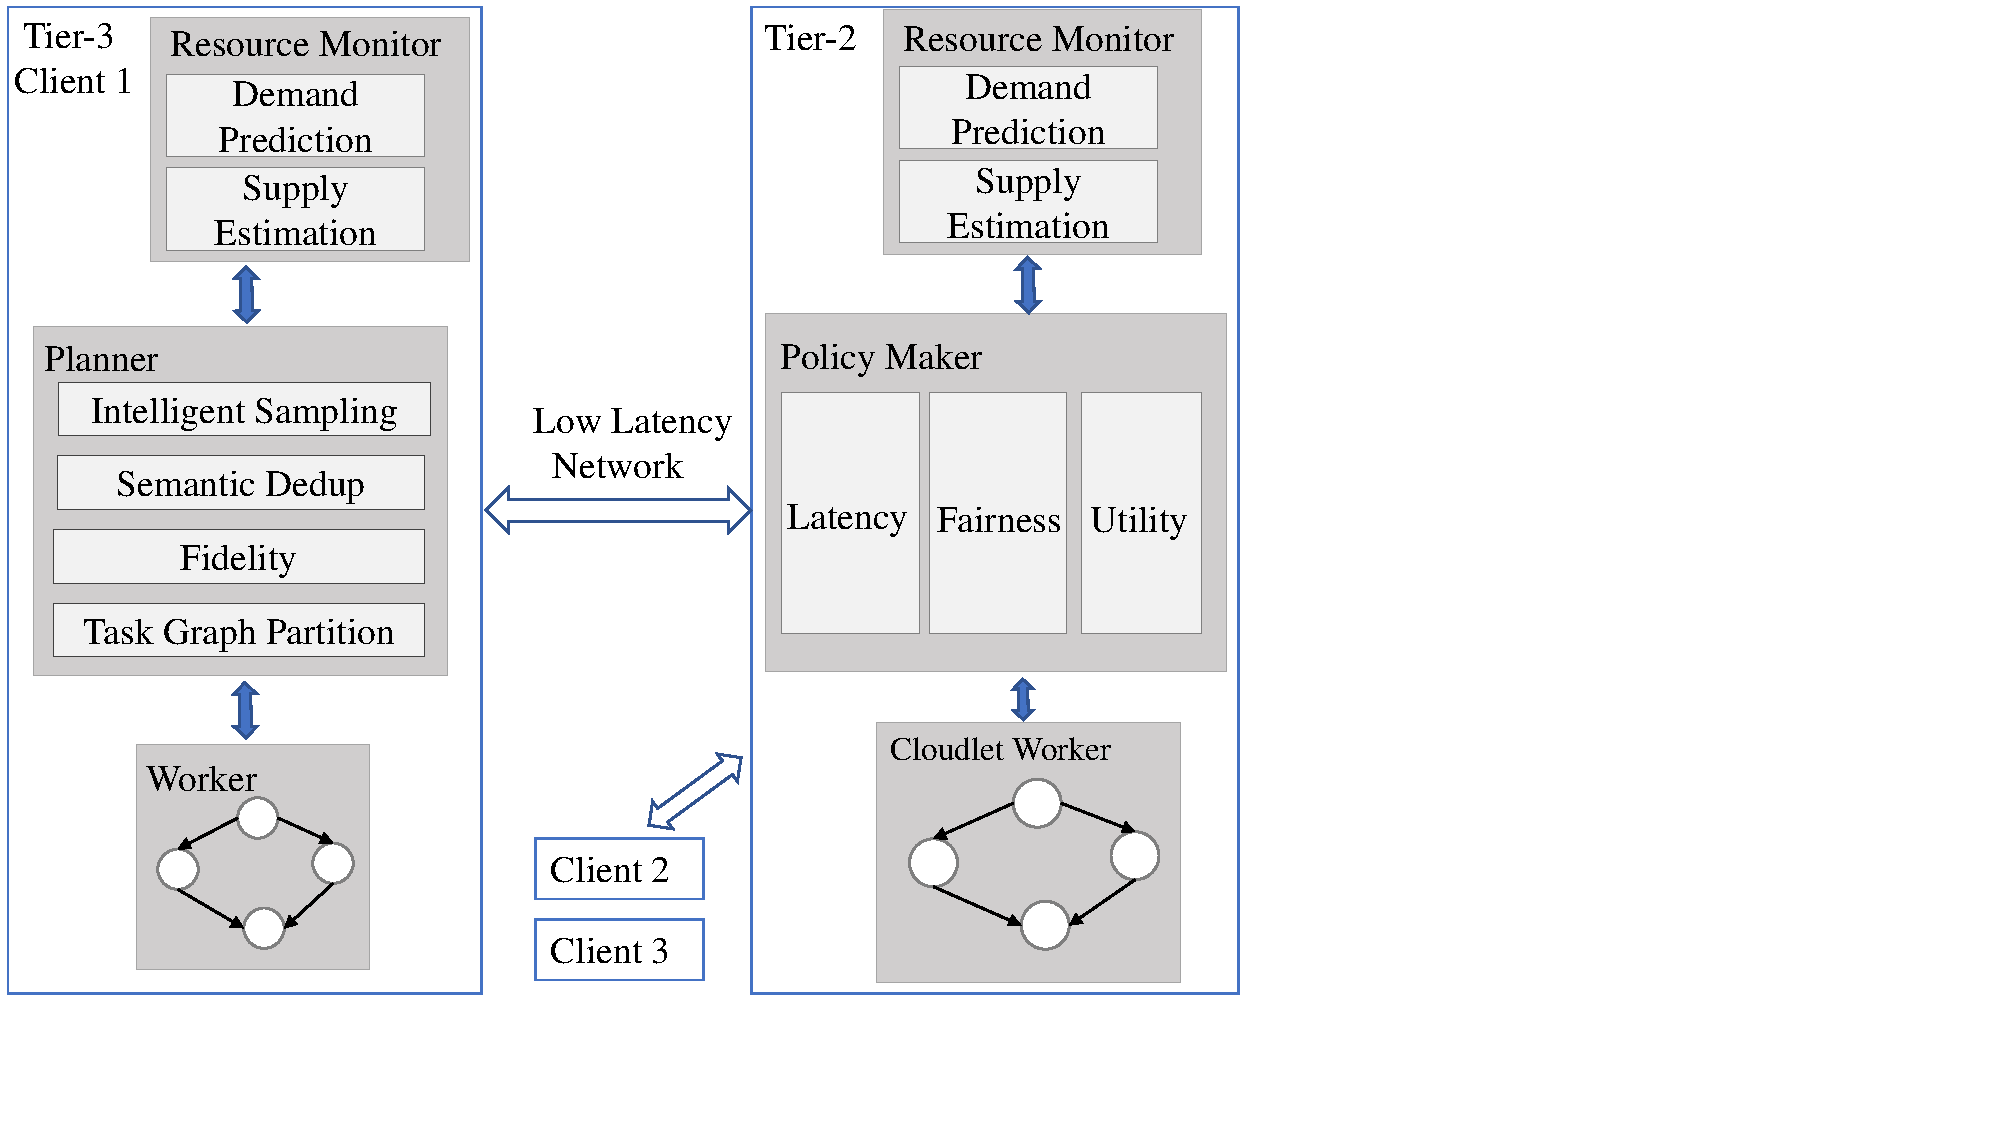
\includegraphics[width=\textwidth,trim=0 3em 11cm 0, clip]{FIGS/arch-vertical.pdf}
\vspace{-0.3in}
\caption{Adaptation Architecture}
\label{fig:arch}
\end{figure}

The original Gabriel platform has been validated in meeting the latency bounds
of WCA applications in single-user settings~\cite{chen2017empirical}.  Scalable
Gabriel aims to meet these latency bounds in multi-user settings, and to ensure
performant multitenancy even in the face of overload.  We take two complementary
approaches to scalability.  The first is for applications to reduce their
offered load to the wireless network and the cloudlet through adaptation.  The
second uses end-to-end scheduling of cloudlet resources to minimize queueing and
impacts of overload (See Chapter~\ref{chapter: cloudlet} for more details).  We
both approaches, and combine them using the system architecture shown in
Figure~\ref{fig:arch}.  We assume benevolent and collaborative clients in the
system.

\section{System Architecture}

Computer vision processing is at the core of wearable cognitive assistance. We
consider scenarios in which multiple Tier-3 devices concurrently offload their
vision processing to a single cloudlet over a shared wireless network.  The
devices and cloudlet work together to adapt workloads to ensure good performance
across all of the applications vying for the limited Tier-2 resources and
wireless bandwidth.  This is reflected in the system architecture shown in
Figure~\ref{fig:arch}.

Monitoring of resources is done at both Tier-3 and Tier-2.  Certain
resources, such as battery level, are device-specific and can only be
monitored at Tier-3.  Other shared resources can only be monitored at
Tier-2: these include processing cores, memory, and GPU.  Wireless
bandwidth and latency are measured independently at Tier-3 and Tier-2,
and aggregated to achieve better estimates of network conditions.

This information is combined with additional high-level predictive knowledge and
factored into scheduling and adaptation decisions.  The predictive knowledge
could arise at the cloudlet (e.g., arrival of a new device, or imminent change
in resource allocations), or at the Tier-3 device (e.g., application-specific,
short-term prediction of resource demand).  All of this information is fed to a
{\em policy module} running on the cloudlet.  This module is guided by an
external policy specification and determines how cloudlet resources should be
allocated across competing Tier-3 applications.  Such policies can factor in
latency needs and fairness, or simple priorities (e.g., a blind person
navigation assistant may get priority over an AR game).

A {\em planner module} on the Tier-3 device uses current resource
utilization and predicted short-term processing demand to determine
which workload reduction techniques (described in
Section~\ref{sec:workload-reduction}) should be applied to achieve
best performance for the particular application given the resource
allocations.

\begin{table*}[]
    \begin{tabular}{|r|p{25ex}|p{30ex}|p{25ex}|}
    \hline&&&\\[0.1in]
    &{\normalsize\bf Question}  & {\normalsize\bf Example} & {\normalsize\bf Load-reduction Technique} \\
    & & & \\ 
    \hline
    1&How often are instructions given, compared to task duration? 
        & Instructions for each step in IKEA lamp assembly are 
            rare compared to the total task time, e.g., 6 instructions over 
            a 10 minute task.
        & Enable adaptive sampling based on active and passive phases. \\ \hline
    2&Is intermittent processing of input frames sufficient for giving instructions?
        & Recognizing a face in any one frame is sufficient for
whispering the person's name.
        & Select and process key frames.  \\ \hline
    3&Will a user wait for system responses before proceeding?  
        & A first-time user of a medical device will pause until  an instruction is received.
        & Select and process key frames. \\ \hline
    4&Does the user have a pre-defined workspace in the scene?
        & Lego pieces are assembled on the lego board. Information outside the board can
             be safely ignored.
        & Focus processing attention on the region of interest. \\ \hline
    5&Does the vision processing involve identifying and locating objects?
        & Identifying a toy lettuce for a toy sandwich.
        & Use tracking as cheap approximation for detection. \\ \hline
    6&Are the vision processing algorithms insensitive to image resolution?
        & Many image classification DNNs limit resolutions to  
            the size of their input layers.
        & Downscale sampled frames on device before transmission.    \\ \hline
    7&Can the vision processing algorithm trade off accuracy and computation? 
        & Image classification DNN MobileNet is computationally cheaper than ResNet, but less accurate. 
        & Change computation fidelity based on resource utilization. \\ \hline
    % 8&Is there inherent human-level latency for a state change?
    %     & It takes at least a few seconds for a human to drill a hole.
    %     & Frame sampling and processing suppression based on heuristics   \\ \hline
    8&Can IMUs be used to identify the start and end of user activities?
        & User's head movement is significantly larger when searching for a Lego block.
        & Enable IMU-based frame suppression. \\ \hline
    9&Is the Tier-3 device powerful enough to run parts of the processing pipeline?
        & A Jetson TX2 can run MobileNet-based image recognition in real-time.
        & Partition the vision pipeline between Tier-3 and Tier-2.   \\ \hline
    \end{tabular}
\vspace{0.1in}
    \caption{Application characteristics and corresponding applicable techniques to reduce load}
    \label{tab:questions-techniques}
\end{table*}

\section{Adaptation Goals}
 
For WCAs, the dominant class of offloaded computations are computer vision
operations, e.g., object detection with deep neural networks (DNNs), or activity
recognition on video segments. The interactive nature of these applications
precludes the use of deep pipelining that is commonly used to improve the
efficiency of streaming analytics.  Here, end-to-end latency of an individual
operation is more important than throughput. Further, it is not just the mean or
median of latency, but also the tail of the distribution that matters.  There is
also significant evidence that user experience is negatively affected by
unpredictable variability in response times. Hence, a small mean with short tail
is the desired ideal. Finally, different applications have varying degrees of
benefit or utility at different levels of latency.  Thus, our adaptation
strategy incorporates application-specific utility as a function of latency as
well as policies maximizing the total utility of the system.


\section{Leveraging Application Characteristics}
\label{sec:workload-reduction}

WCA applications exhibit certain properties that distinguish them from
other video analytics applications studied in the past.  Adaptation
based on these attributes provides a unique opportunity to improve
scalability.

\textbf{Human-Centric Timing:} The frequency and speed with which guidance must
be provided in a WCA application often depends on the speed at which the human
performs a task step.  Generally, additional guidance is not needed until the
instructed action has been completed. For example, in the RibLoc assistant
(Chapter~\ref{chapter: background}), drilling a hole in bone can take several
minutes to complete.  During the drilling, no further guidance is provided after
the initial instruction to drill.  Inherently, these applications contain {\em
active phases,} during which an application needs to sample and process video
frames as fast as possible to provide timely guidance, and {\em passive phases,}
during which the human user is busy performing the instructed step.  During a
passive phase, the application can be limited to sampling video frames at a low
rate to determine when the user has completed or nearly completed the step, and
may need guidance soon.  Although durations of human operations need to be
considered random variables, many have empirical lower bounds.  Adapting
sampling and processing rates to match these active and passive phases can
greatly reduce offered load.  Further, the offered load across users is likely
to be uncorrelated because they are working on different tasks or different
steps of the same task. If inadvertent synchronization occurs, it can be broken
by introducing small randomized delays in the task guidance to different users.
These observations suggest that proper end-to-end scheduling can enable
effective use of cloudlet resources even with multiple concurrent applications.

\textbf{Event-Centric Redundancy}: In many WCA applications, guidance
is given when a user event causes visible state change. For example,
placing a lamp base on a table triggers the IKEA Lamp application to
deliver the next assembly instruction.  Typically, the application
needs to process video at high frame rate to ensure that such state
change is detected promptly, leading to further guidance.  However,
all subsequent frames will continue to reflect this change, and are
essentially redundant, wasting wireless and computing resources.
Early detection of redundant frames through careful semantic
deduplication and frame selection at Tier-3 can reduce the use of
wireless bandwidth and cloudlet cycles on frames that show no
task-relevant change.

\textbf{Inherent Multi-Fidelity}: Many vision processing algorithms
can tradeoff fidelity and computation.  For example, frame resolution
can be lowered, or a less sophisticated DNN used for inference, in
order to reduce processing at the cost of lower accuracy.  In many
applications, a lower frame rate can be used, saving computation and
bandwidth at the expense of response latency.  Thus, when a cloudlet
is burdened with multiple concurrent applications, there is scope to
select operating parameters to keep computational load manageable.
Exactly how to do so may be application-dependent.  In some cases,
user experience benefits from a trade-off that preserves fast response
times even with occasional glitches in functionality.  For others,
e.g., safety-critical applications, it may not be possible to
sacrifice latency or accuracy.  This in turn, translates to lowered
scalability of the latter class of application, and hence the need for
a more powerful cloudlet and possibly different wireless technology to
service multiple users.

\begin{figure}[h]
    \centering
    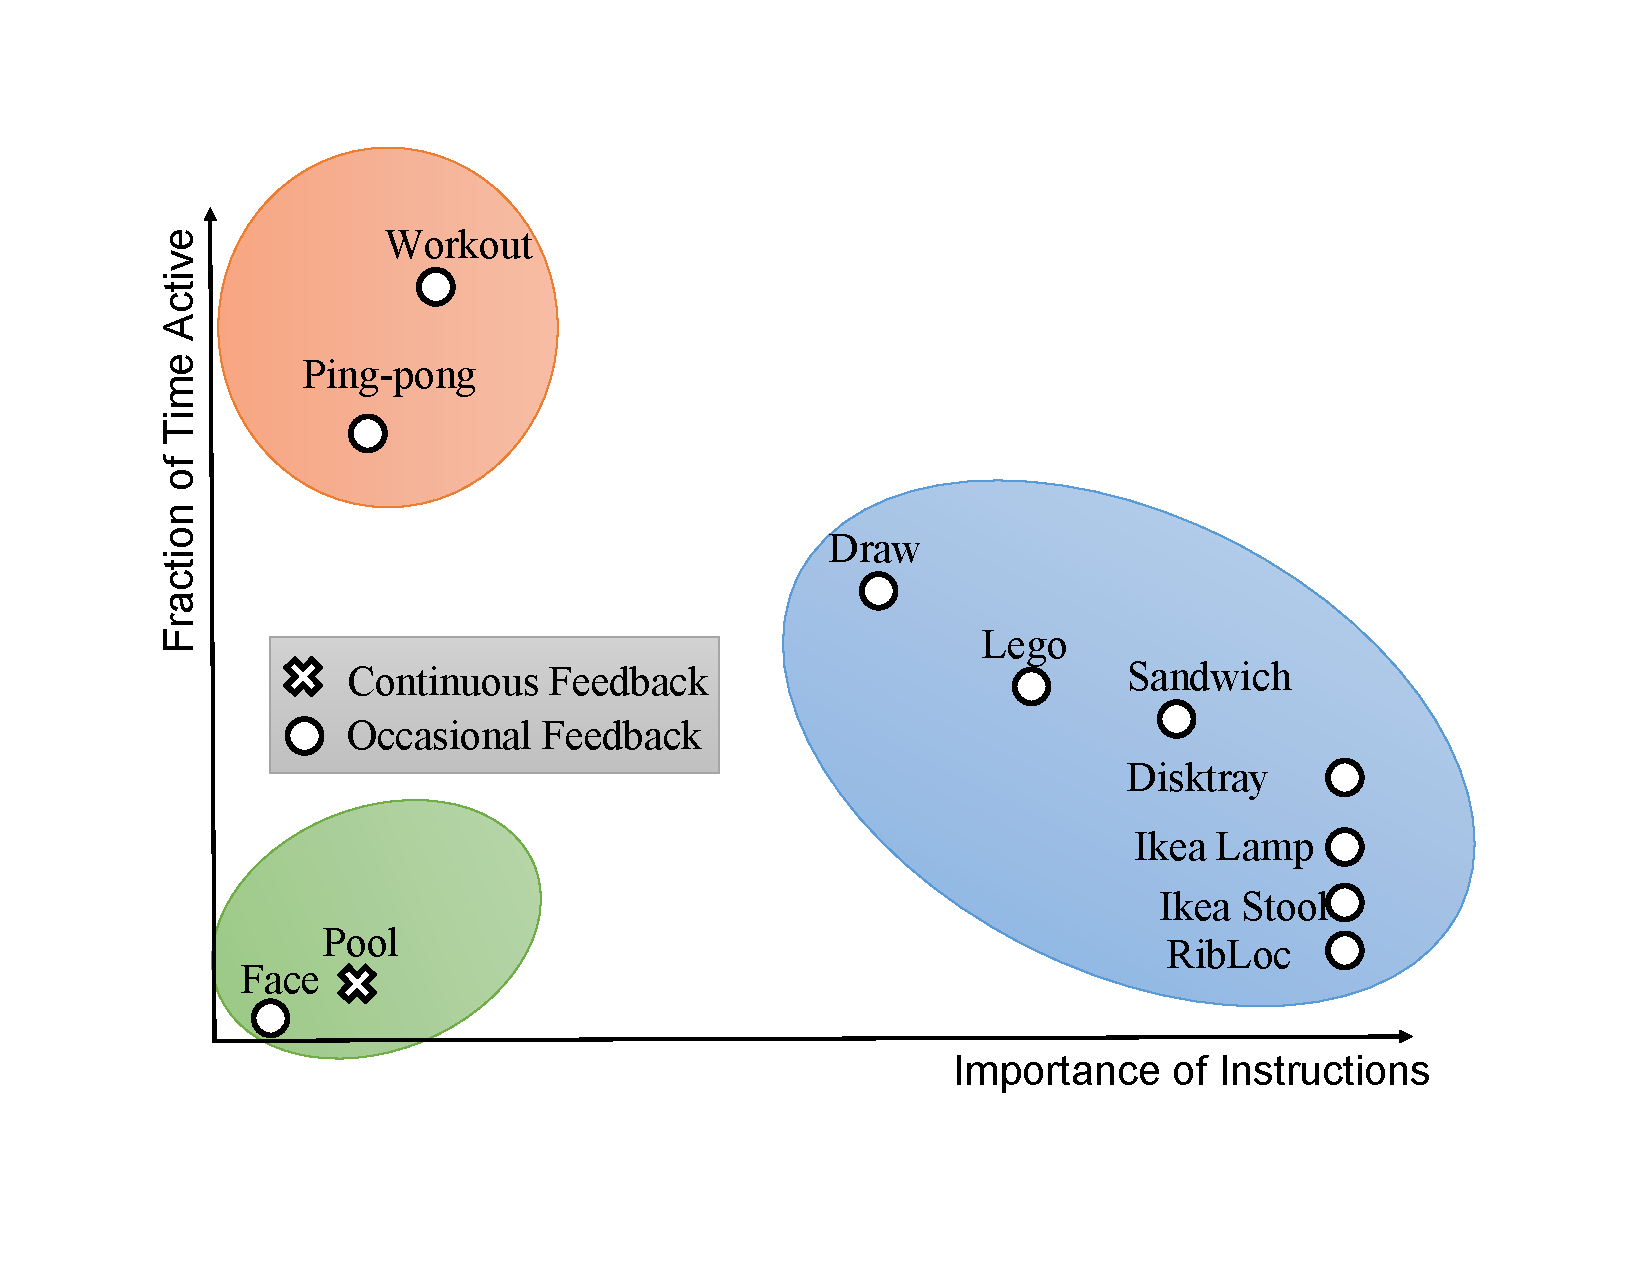
\includegraphics[width=\linewidth, trim=10em 2em 6em 2em, clip]{FIGS/fig-design-space.pdf}
    \caption{Design Space of WCA Applications}
    \label{figs:design-space}
\end{figure}
\subsection{Adaptation-Relevant Taxonomy}

\label{sec:taxonomy}

The characteristics described in the previous section largely hold for
a broad range of WCA applications.  However, the degree to which
particular aspects are appropriate to use for effective adaptation is
very application dependent, and requires a more detailed
characterization of each application.  To this end, our system
requests a manifest describing an application from the developers.
This manifest is a set of yes/no or short numerical responses to the
questions in Table~\ref{tab:questions-techniques}.  Using these, we
construct a taxonomy of WCA applications (shown in
Figure~\ref{figs:design-space}), based on clusters of applications along
dimensions induced from the checklist of questions.  In this case, we
consider two dimensions -- the fraction of time spent in "active"
phase, and the significance of the provided guidance (from merely
advisory, to critical instructions).  Our system varies the adaptation
techniques employed to the different clusters of applications.  We
note that as more applications and more adaptation techniques are
created, the list of questions can be extended, and the taxonomy can be
expanded.

\section{Adaptive Sampling}

The processing demands and latency bounds of a WCA application can
vary considerably during task execution because of human speed
limitations.  When the user is awaiting guidance, it is desirable to
sample input at the highest rate to rapidly determine task state and
thus minimize guidance latency.  However, while the user is performing
a task step, the application can stay in a passive state and sample at
a lower rate.  For a short period of time immediately after guidance
is given, the sampling rate can be very low because it is not humanly
possible to be done with the step.  As more time elapses, the
sampling rate has to increase because the user may be nearing
completion of the step.  Although this active-passive phase
distinction is most characteristic of WCA applications that provide
step-by-step task guidance (the blue cluster in
the lower right of Figure~\ref{figs:design-space}), most WCA
applications exhibit this behavior to some degree.  As shown in the
rest of this section, adaptive sampling rates can reduce processing
load without impacting application latency or accuracy.

We use task-specific heuristics to define application active and
passive phases.  In an active application phase, a user is likely to
be waiting for instructions or comes close to needing instructions,
therefore application needs to be ``active`` by sampling and
processing at high frequencies. On the other hand, applications can
run at low frequency during passive phases when an instruction is
unlikely to occur.

\begin{figure}
\centering
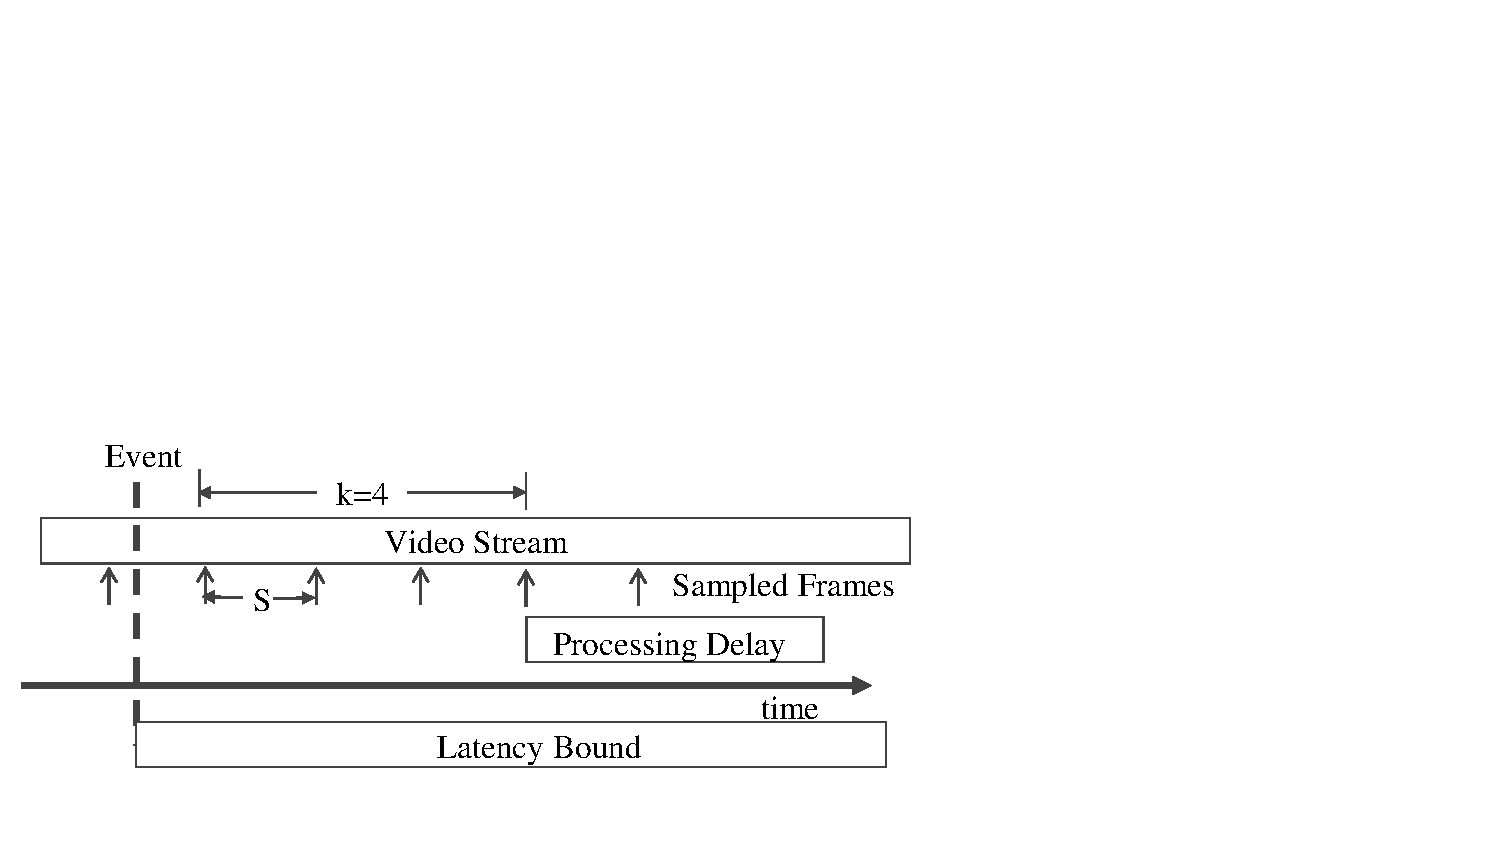
\includegraphics[width=\textwidth,trim=0em 3em 20em 15em, clip]{FIGS/fig-lego-sampling-model.pdf}
\caption{\small Dynamic Sampling Rate for LEGO}
\label{fig:lego-sampling-model}
\end{figure}

We use the LEGO application from Section~\ref{sec:example-apps} to show the
effectiveness of adaptive sampling. By default, the LEGO application runs at
active phase. The application enters passive phases immediately following the
delivery of an instruction, since the user is going to take a few seconds
searching and assembling LEGO blocks. The length and sampling rate of a passive
phase is provided by the application to the framework. We provide the following
system model as an example of what can be provided. We collect five LEGO traces
with 13739 frames as our evaluation dataset.

\textbf{Length of a Passive Phase: }
We model the time it takes to finish each step as a Gaussian distribution. We
use maximum likelihood estimation to calculate the parameters of the Guassian
model.

 
\begin{figure}
\small\centering
\begin{subfigure}{.45\linewidth}
  \centering
  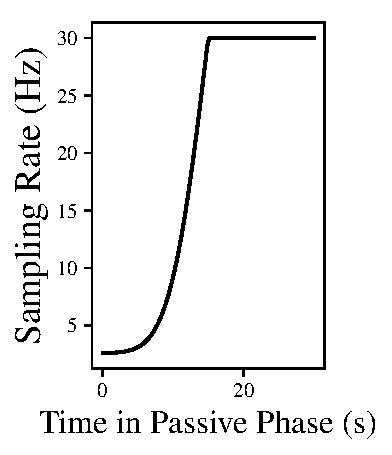
\includegraphics[width=\linewidth, trim=0em 0em 0em 0em, clip]{FIGS/fig-lego-adaptive-sr.pdf}
  {\small (a) Passive Sampling Rate}
\end{subfigure}
\begin{subfigure}{.45\linewidth}
    \centering
    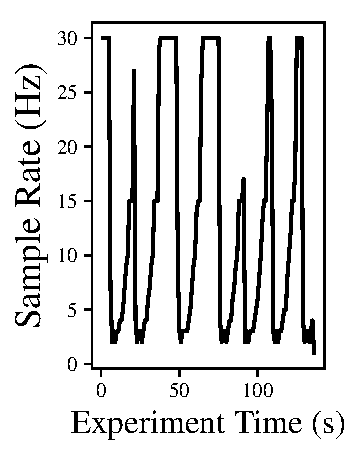
\includegraphics[width=0.92\linewidth, trim=0em 0em 0em 0em, clip]{FIGS/fig-lego-example-sr.pdf}
   {\small (b) Trace Sampling Rate}
\end{subfigure}
\caption{\small Adaptive Sampling Rate}
\label{fig:adaptive-sampling-example}
\end{figure}

\textbf{Lowest Sampling Rate in Passive Phase: }
The lowest sampling rate in passive phase still needs to meet application's
latency requirement. Figure~\ref{fig:lego-sampling-model} shows the system model
to calculate the largest sampling period S that still meets the latency bound.
In particular,
$$(k-1)S + processing\_delay \leq latency\_bound $$ $k$ represents the
cumulative number of frames an event needs to be detected in order to be
certain an event actually occurred. The LEGO application empirically sets this
value to be 5. 

\textbf{Adaptation Algorithm: }
At the start of a passive phase, we set the sampling rate to the
minimum calculated above.  As time progresses, we gradually increase
the sampling rate.  The idea behind this is that the initial low
sampling rates do not provide good latency, but this is acceptable, as
the likelihood of an event is low.  As the likelihood increases (based
on the Gaussian distribution described earlier), we increase sampling
rate to decrease latency when events are likely.
Figure~\ref{fig:adaptive-sampling-example}(a) shows the sampling rate
adaptation our system employs during a passive phase.
The sampling rate is calculated as $$sr = \\
%
 min\_sr + \alpha * (max\_sr - min\_sr) * cdf\_Gaussian(t)$$ 
%
$sr$ is the sampling rate. $t$ is the time after an instruction has been given. $\alpha$ is
a recovery factor which determines how quickly the sampling rate
rebounds to active phase rate. 


Figure~\ref{fig:adaptive-sampling-example}(b) shows the sampling rate
for a trace as the application runs. The video captures a user doing 7
steps of a LEGO assembly task. Each drop in sampling rate happens
after an instruction has been delivered to the user.
Table~\ref{tab:adaptive-sample-eval} shows the percentage of frames
sampled and guidance latency comparing adaptive sampling with naive
sampling at half frequency. Our adaptive sampling scheme requires
processing fewer frames while achieving a lower guidance latency.

\begin{table}[]
\small\centering
\begin{tabular}{|c|c|c|}
\hline
Trace  & \begin{tabular}[c]{@{}c@{}}Sample\\ Half Freq\end{tabular} & \begin{tabular}[c]{@{}c@{}}Adaptive\\ Sampling\end{tabular} \\ \hline
1 & 50\%          & 25\%              \\ \hline
2 & 50\%          & 28\%              \\ \hline
3 & 50\%          & 30\%              \\ \hline
4 & 50\%          & 30\%              \\ \hline
5 & 50\%          & 43\%              \\ \hline
\end{tabular}\\[0.1in]
{\small (a) Percentage of Frames Sampled}\\[0.2in]

\begin{tabular}{|c|c|}
\hline
                                                            & \begin{tabular}[c]{@{}c@{}}Guidance Delay \\ (frames$\pm$stddev)\end{tabular}
                                                            \\ \hline
\begin{tabular}[c]{@{}c@{}}Sample Half Freq\end{tabular}      & 7.6 $\pm$ 6.9                                                                  \\ \hline
\begin{tabular}[c]{@{}c@{}}Adaptive Sampling\end{tabular} &  5.9 $\pm$ 8.2                                                                  \\ \hline
% \begin{tabular}[c]{@{}c@{}}Theoretical Minimum\end{tabular} &  ?? $$                                                                  \\ \hline
\end{tabular}\\[0.1in]
{\small (b) Guidance Latency}\\[0.1in]
\caption{\small Frames Sampled and Guidance Latency}
\label{tab:adaptive-sample-eval}
\vspace{-0.2in}
\end{table}
\section{IMU-based Approaches: Passive Phase Suppression}

% comment: add image quality evaluation?

\begin{figure}[h]
\begin{center}
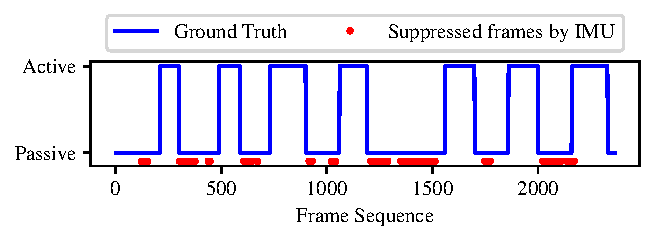
\includegraphics[width=.9\linewidth]{FIGS/fig-imu-trace-lego.pdf}\\
{\small (a) LEGO}
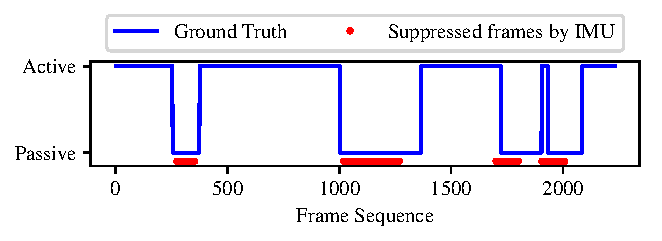
\includegraphics[width=.9\linewidth]{FIGS/fig-imu-trace-pingpong.pdf}\\
{\small (b) PING PONG}
\end{center}
\vspace{-0.1in}
\caption{\small Accuracy of IMU-based Frame Suppression}
\label{fig:imu-trace-example}
\vspace{-0.1in}
\end{figure}

In many applications, passive phases can often be associated with the
user's head movement. We illustrate with two applications here. In
LEGO, during the passive phase, which begins after the user receives
the next instruction, a user typically turns away from the LEGO board
and starts searching for the next brick to use in a parts box. During
this period, the computer vision algorithm would detect no meaningful
task states if the frames are transmitted.  In PING PONG, an active
phase lasts throughout a rally.  Passive phases are in between actual
game play, when the user takes a drink, switches sides, or, most
commonly, tracks down and picks up a wayward ball from the floor.
These are associated with much large range of head movements than
during a rally when the player generally looks toward the opposing
player.  Again, the frames can be suppressed on the client to reduce
wireless transmission and load on the cloudlet.  In both scenarios,
significant body movement can be detected through Inertial Measurement
Unit (IMU) readings on the wearable device, and used to predict those
passive phases.

For each frame, we get a six-dimensional reading from the IMU:
rotation in three axes, and acceleration in three axes.  We train an
application-specific SVM to predict active/passive phases based on IMU
readings, and suppress predicted passive frames on the client.
Figure~\ref{fig:imu-trace-example}(a) and (b) show an example trace
from LEGO and PING PONG, respectively.  Human-labeled ground truth
indicating passive and active phases is shown in blue.  The red dots
indicate predictions of passive phase frames based on the IMU
readings; these frames are suppressed at the client and not
transmitted.  Note that in both traces, the suppressed frames also
form streaks. In other words, a number of frames in a row can be
suppressed. As a result, the saving we gain from IMU is orthogonal to
that from adaptive sampling.

Although the IMU approach does not capture all of the passive frames
(e.g., in LEGO, the user may hold his head steady while looking for
the next part), when a passive frame is predicted, this is likely
correct (i.e., high precision, moderate recall).  Thus, we expect
little impact on event detection accuracy or latency, as few if any
active phase frames are affected.  This is confirmed in
Table~\ref{tab:imu-result}, which summarizes results for five traces
from each application.  We are able to suppress up to 49.9\% of
passive frames for LEGO and up to 38.4\% of passive frames in case of
PING PONG on the client, while having minimal impact on application
quality --- incurring no delay in state change detection in LEGO, and
less than 2\% loss of active frames in PING PONG.

\begin{table}[h]
\small\centering
\begin{tabular}{| l | c | c |}
   \hline
        & Suppressed  &  Max Delay of \\ 
        & Passive Frames (\%)   & State Change Detection \\ \hline
    Trace 1 & 17.9\%    & 0 \\
    Trace 2 & 49.9\%    & 0 \\
    Trace 3 & 27.1\%    & 0 \\
    Trace 4 & 37.0\%    & 0 \\
    Trace 5 & 34.1\%    & 0 \\
    \hline
\end{tabular}\\[0.1in]
{\small (a) LEGO}\\[0.1in]

\begin{tabular}{| l | c | c |}
    \hline
        & Suppressed        & Loss of  \\
        & Passive Frames (\%)    & Active Frames (\%) \\ \hline
    Trace 1 & 21.5\%    &   0.8\%   \\
    Trace 2 & 30.0\%    &   1.5\%   \\
    Trace 3 & 26.2\%    &   1.9\%   \\
    Trace 4 & 29.8\%    &   1.0\%   \\
    Trace 5 & 38.4\%    &   0.2\%   \\
    \hline
\end{tabular}\\[0.1in]
{\small (b) PING PONG}\\[0.1in]
\caption{\small Effectiveness of IMU-based Frame Suppression}
\label{tab:imu-result}
\end{table}

\section{Related Work}
\label{sec: workload-related}

Although edge computing is new, the techniques for reducing offered load to
adapt application behaviors examined in this chapter bear some resemblance to
work that was done in the early days of mobile computing.

Several different approaches to adapting application fidelity have been studied.
Dynamic sampling rate with various heuristics for adaptation have been tried
primarily in the context of individual mobile devices for energy
efficiency~\cite{lorincz2009mercury, lorincz2008resource, vallina2012energy,
lane2010survey}. Semantic deduplication to reduce redundant processing of frames
have been suggested by ~\cite{Hu2015, kang2017noscope, hsieh2018focus,
zhang2015design}. Similarly, previous works have looked at suppression based on
motion either from video content~\cite{naderiparizi2017glimpse,
lebeckcollaborative} or IMUs~\cite{jain2015overlay}. Others have investigated
exploiting multiple deep models with accuracy and resource
tradeoffs~\cite{han2016mcdnn,jiang2018chameleon}. In addition, using tracking as
approximate result of detection and recognition has been explored to leverage
the temporal locality of video data and reduce computational
demand~\cite{wang2017scalable, chen2015glimpse, you1999hybrid}. While most of
these efforts were in mobile-only, cloud-only, or mobile-cloud context, we
explore similar techniques in an edge-native context.


Partitioning workloads between mobile devices and the cloud have been
studied in sensor networks~\cite{newton2009wishbone},
throughput-oriented systems~\cite{cuervo2010maui, yi2017lavea}, for
interactive applications~\cite{ra2011odessa, chen2015glimpse}, and
from programming model perspectives~\cite{balan2003tactics}. We believe
that these approaches will become important techniques to scale
applications on heavily loaded cloudlets.

\section{Chapter Summary and Discussion}
\label{sec:workload-reduction-summary}

In this chapter, we demonstrate that scalability can be increased by leveraging
application characteristics to reduce offered load. Our approach to increased
scalability is through adaptation. Specifically, we first present an
adaptation-centric architecture that monitors and coordinates Tier-3 devices and
the edge server. When contention arises, enabled are application-specific
optimizations to reduce offered load to the edge server. In addition, we highlight
two of adaptation techniques, selective sampling and IMU-based suppression. Our
experiment show that they can significantly reduce the offered load. Finally, we
provide a taxonomy to help developers reason about characteristics of their
applications, and identify and specify reduction techniques applicable to their
needs.
